\section{Auswertung}
\label{sec:auswertung}

	\subsection{Brechungsindizes $n_\mathrm{i}$ in Abh"angigkeit der Wellenl"ange $\lambda$}
	\label{subsec:brechungsindizes}
		Zun"achst werden aus den Messdaten, die in Tabellen \ref{table:phi} und \ref{table:eta} aufgef"uhrt sind, die Winkel $\varphi$ und $\eta$ bestimmt.
		Die Mittelung "uber die Daten aller Wellenl"angen $\lambda$ liefert mit Gleichung \eqref{eqn:phi}:

		\begin{equation*}
			\varphi = \SI{69.7 (11)}{\degree} \,.
		\end{equation*}

		Aus dem Versuchsaufbau geht jedoch hervor, dass alle Winkel des Prismas etwa $\varphi = \SI{60}{\degree}$ betragen m"ussen.
		Weil dieser Wert den tats"achlichen Aufbau des Prismas offensichtlich besser wiederspiegelt, wird im Folgenden damit weitergerechnet.
		Die resultierenden Werte der Brechungsindizes wird mit $n_\mathrm{opt}$ gekennzeichnet.
		Auf die Abweichung des gemessenen Wertes zum optimalen Wert wird in der Diskussion (\ref{sec:diskussion}) eingegangen.

		Die Messwerte liefern anschlie"send mit Gleichung \eqref{eqn:brechungsindex} die in Tabelle \ref{table:brechungsindizes} aufgef"uhrten Brechungsindizes $n_\mathrm{opt}$ und $n$:

		\begin{table}[h!]
			\begin{center}
				\caption{Werte des Brechungsindex bei verschiedenen Wellenl"angen $\lambda$ \label{table:brechungsindizes}}
				\begin{tabular}{|c|c|c|c|}
					\hline
						Farbe & $\lambda [\SI{}{\nano \meter}]$ & $n_\mathrm{opt}$ & $n$ \\
					\hline 
					\hline
						gelb & $\SI{578.0}{}$ & $\SI{1.657}{}$ & $\SI{1.528}{}$ \\
						gr"un & $\SI{546.1}{}$ & $\SI{1.652}{}$ & $\SI{1.524}{}$ \\
						blaugr"un & $\SI{591.6}{}$ & $\SI{1.645}{}$ & $\SI{1.519}{}$ \\
						violett & $\SI{404.7}{}$ & $\SI{1.634}{}$ & $\SI{1.511}{}$ \\
						ultraviolett & $\SI{365.0}{}$ & $\SI{1.627}{}$ & $\SI{1.505}{}$ \\
						ultraviolett & $\SI{366.3}{}$ & $\SI{1.625}{}$ & $\SI{1.504}{}$ \\
					\hline 
				\end{tabular}
			\end{center}
		\end{table}

		\begin{table}[h!]
			\begin{center}
				\caption{Messwerte zur Bestimmung von $\varphi$ \label{table:phi}}
				\begin{tabular}{|c|c|c|c|c|}
					\hline
						Farbe & $\lambda [\SI{}{\nano \meter}]$ & $\varphi_\mathrm{l} [\SI{}{\degree}]$ & $\varphi_\mathrm{r} [\SI{}{\degree}]$ & $\varphi [\SI{}{\degree}]$ \\
					\hline 
					\hline
						gelb         & $\SI{578.0}{}$ & $\SI{97.2}{}$ & $\SI{239.2}{}$ & $\SI{71.0}{}$\\
gr"un        & $\SI{546.1}{}$ & $\SI{97.8}{}$ & $\SI{239.0}{}$ & $\SI{70.6}{}$\\
blaugr"un    & $\SI{591.6}{}$ & $\SI{98.0}{}$ & $\SI{238.4}{}$ & $\SI{70.2}{}$\\
violett      & $\SI{404.7}{}$ & $\SI{99.0}{}$ & $\SI{237.6}{}$ & $\SI{69.3}{}$\\
ultraviolett & $\SI{365.0}{}$ & $\SI{99.4}{}$ & $\SI{236.4}{}$ & $\SI{68.5}{}$\\
ultraviolett & $\SI{366.3}{}$ & $\SI{99.6}{}$ & $\SI{236.2}{}$ & $\SI{68.3}{}$\\
					\hline 
				\end{tabular}
			\end{center}
		\end{table}		

		\begin{table}[h!]
			\begin{center}
				\caption{Messwerte zur Bestimmung von $\eta$ \label{table:eta}}
				\begin{tabular}{|c|c|c|c|c|}
					\hline
						Farbe & $\lambda [\SI{}{\nano \meter}]$ & $\Omega_\mathrm{l} [\SI{}{\degree}]$ & $\Omega_\mathrm{r} [\SI{}{\degree}]$ & $\eta [\SI{}{\degree}]$ \\
					\hline 
					\hline
						gelb         & $\SI{578.0}{}$ & $\SI{53.4}{}$ & $\SI{285.3}{}$ & $\SI{51.9}{}$ \\
gr"un        & $\SI{546.1}{}$ & $\SI{53.6}{}$ & $\SI{285.0}{}$ & $\SI{51.4}{}$ \\
blaugr"un    & $\SI{491.6}{}$ & $\SI{54.0}{}$ & $\SI{284.7}{}$ & $\SI{50.7}{}$ \\
violett      & $\SI{404.7}{}$ & $\SI{54.5}{}$ & $\SI{284.1}{}$ & $\SI{49.6}{}$ \\
ultraviolett & $\SI{365.0}{}$ & $\SI{54.9}{}$ & $\SI{283.8}{}$ & $\SI{48.9}{}$ \\
ultraviolett & $\SI{366.3}{}$ & $\SI{55.0}{}$ & $\SI{283.7}{}$ & $\SI{48.7}{}$ \\
					\hline 
				\end{tabular}
			\end{center}
		\end{table}		

	\clearpage

	\subsection{Bestimmung der Dispersionsgleichung und deren Parameter $A_\mathrm{i}$}
	\label{subsec:dispersionskurve}
		Es werden zwei nichtlineare Ausleichsrechung der $\lambda$- $n^2$- Wertepaare, f"ur Dispersiosngleichungen \eqref{eqn:dispersion1} und \eqref{eqn:dispersion2} durchgef"uhrt.
		Die Ausgleichsrechnung liefert die Koeffizienten $A_\mathrm{i}$ und $A'_\mathrm{i}$, sowie deren Fehler $\Delta A$.

		Daraus lassen sich die Abweichungsquadrate bei einer Anzahl von $z$ Messwerten wie folgt berechnen:

		\begin{eqnarray*}
			s^2 & = & \frac{1}{z - 2} \sum_{\mathrm{i} = 1}^z{\left(n^2(\lambda_\mathrm{i}) - A_0 - \frac{A_2}{\lambda_\mathrm{i}^2}\right)^2} \,, \\
			s'^2 & = & \frac{1}{z - 2} \sum_{\mathrm{i} = 1}^z{\left(n^2(\lambda_\mathrm{i}) - A'_0 + A'_2 \cdot \lambda_\mathrm{i}^2 \right)^2} \,. \\
		\end{eqnarray*}

		Die Ausgleichsrechnung liefert die Koeffizienten

		\begin{eqnarray*}
			A_0 = \SI{2.65 (9)}{} && \,, \\
			A_2 = \SI{-8.25(4096)e-15}{\meter \tothe{2}} && A'_2 = \SI{-6.14e12}{} \pm \infty \,, \\
			A_4 = \SI{2.60(395)e-27}{\meter \tothe{4}} && A'_4 = \SI{1}{} \pm \infty \,. \\
		\end{eqnarray*}

		Bei den gestrichenen Koeffizienten ist zu bemerken, dass der Fehler die Gr"o"senbegrenzng des Rechnerspeichers f"ur Flie"skommazahlen erreicht hat und daher einen unendlichen Wert liefert.
		Dieser Wert hat keine physikalische Bedeutung, deutet aber schon darauf hin, dass die entsprechende Dispersionsgleichung nicht in der Lage ist, den vorliegenden Aufbau zu beschreiben.
		Das wird deutlicher, wenn man die Abweichungsquadrate berechnet:

		\begin{eqnarray*}
			s^2 & = & \SI{.0136}{} \,, \\
			s'^2 & = & \SI{5.66e25}{} \,. \\
		\end{eqnarray*}

		Weil die Abweichung $s'^2$ f"ur Gleichung \eqref{eqn:dispersion2} gr"o"ser, als $s^2$ ist, wird die hier auftretende Dispersion durch Gleichung \eqref{eqn:dispersion1} beschrieben.
		Die folgenden Abbildungen zeigen die Messwerte, sowie den Verlauf der Dispersionsgleichung.

		\begin{figure}[h]
			\centering
			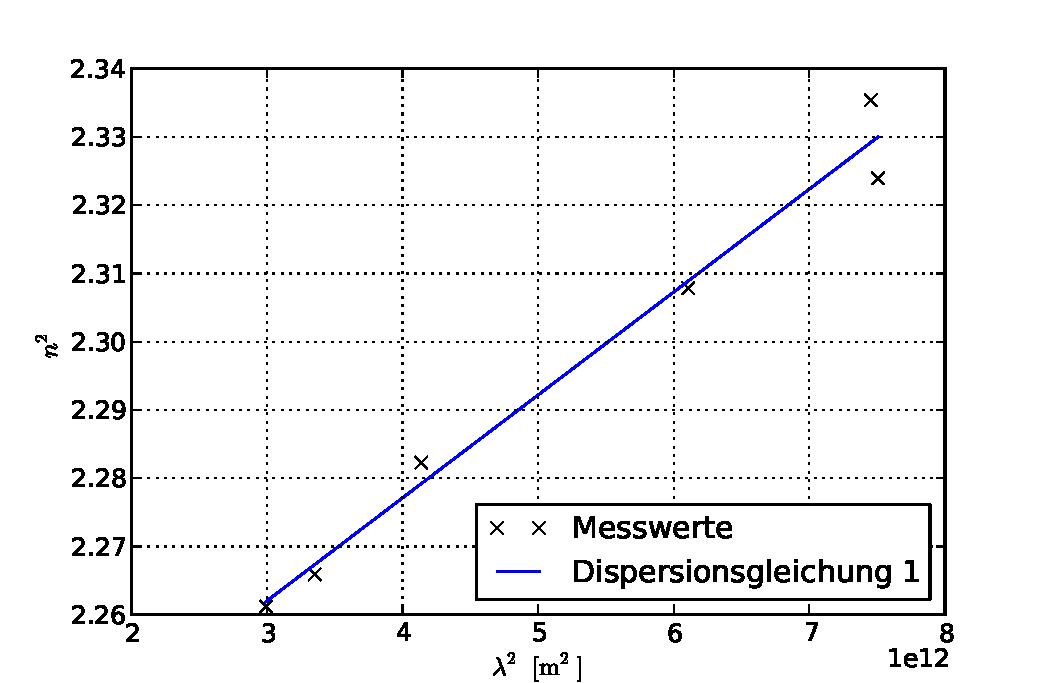
\includegraphics[width = 15cm]{img/dispersion1.pdf}
			\caption{Ausgleichskurve mit Hilfe von Gleichung \eqref{eqn:dispersion1} \label{fig:dispersion1}}
		\end{figure}

		\begin{figure}[h]
			\centering
			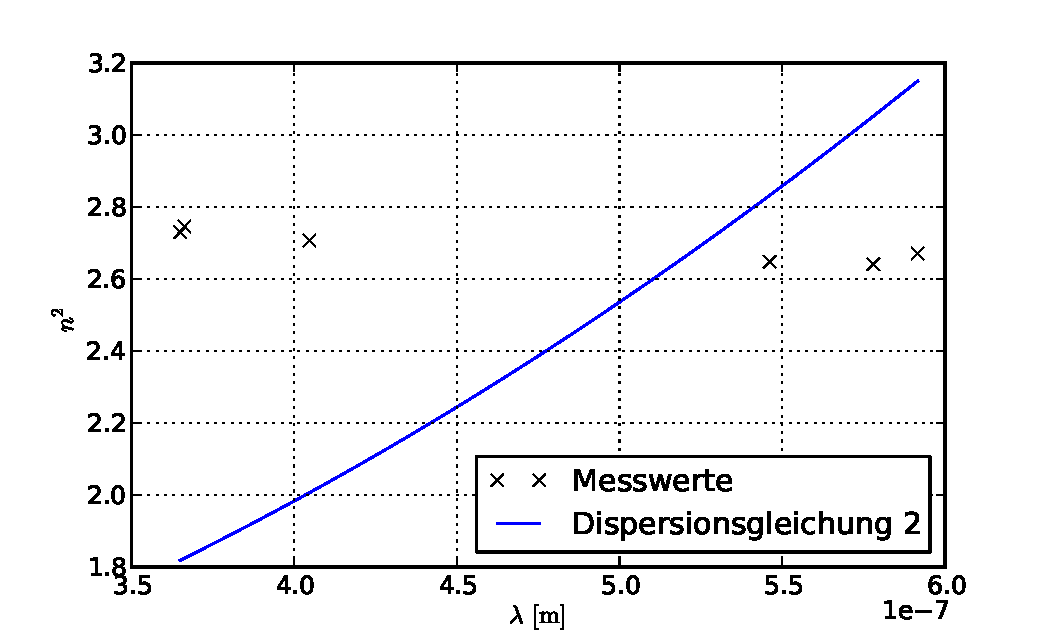
\includegraphics[width = 15cm]{img/dispersion2.pdf}
			\caption{Ausgleichskurve mit Hilfe von Gleichung \eqref{eqn:dispersion2} \label{fig:dispersion2}}
		\end{figure}

	\clearpage

	\subsection{Berechnung der Abbeschen Zahl $\nu$}
	\label{subsec:abbe}
		Mit Gleichung \eqref{eqn:abbe} und Kenntnis der Koeffizienten $A_0$ bis $A_4$ aus Kapitel \ref{subsec:dispersionskurve} l"asst sich die Abbesche Zahl bestimmen.
		Die Dispersionsgleichung liefert zun"achst

		\begin{eqnarray*}
			n_\mathrm{C} & = & \SI{1.6278}{} \,, \\
			n_\mathrm{D} & = & \SI{1.6288}{} \,, \\
			n_\mathrm{F} & = & \SI{1.6330}{} \,. \\
		\end{eqnarray*}

		Daraus folgt

		\begin{equation*}
			\nu = \SI{121.5}{} \,.
		\end{equation*}

	\subsection{Das Aufl"osungsverm"ogen $A$ des Prismas}
	\label{subsec:aufloesungsvermoegen}
		Wie in Kapitel \ref{sec:durchfuehrung} gezeigt, gilt mit einer Basisbreite $b$ des Prismas f"ur das Aufl"osungsverm"ogen:

		\begin{equation*}
			A = \frac{\lambda}{\Delta \lambda} = b \frac{\partial n}{\partial \lambda} \,.
		\end{equation*}

		Mit der hier genutzten Dispersionsgleichung \eqref{eqn:dispersion1} folgt

		\begin{equation*}
			A = b \left( \frac{2A_2}{\lambda^3} + \frac{4A_4}{\lambda^5} \right) \,.
		\end{equation*}

		Bei einer Basisl"ange $b = \SI{3}{\centi \meter}$ folgt f"ur das Aufl"osungsverm"ogen des hier vorliegenden Prismas bei den Fraunhoferwellenl"angen $\lambda_\mathrm{C} = \SI{656}{\nano \meter}$ und $\lambda_\mathrm{F} = \SI{486}{\nano \meter}$:

		\begin{eqnarray*}
			A_\mathrm{C} & = & \SI{820}{} \,, \\
			A_\mathrm{F} & = & \SI{7216}{} \,. \\
		\end{eqnarray*}

		\clearpage

	\subsection{Berechnung des n"achsten Absorptionspunktes $\lambda_\mathrm{1}$}
	\label{subsec:absorptionspunkt}
		Durch Koeffizientenvergleich in Formeln \eqref{eqn:dispersion1} und \eqref{eqn:dispersion1exakt} erh"alt man

		\begin{eqnarray*}
			A_0 & = & 1 + \frac{N_1 q_1^2 \lambda_1^2}{4 \pi^2 c^2 \epsilon_0 m_1} \,, \\
			A_2 & = & \lambda_1^2 (A_0 - 1) \,, \\
			A_4 & = & \lambda_1^4 (A_0 - 1) \,, \\
			\Rightarrow \quad \lambda_1 & = & \sqrt{\frac{A_2}{A_0 - 1}} \,, \\
			\lambda_1 & = & \left(\frac{A_4}{A_0 - 1}\right)^\frac{1}{4} \,. \\
		\end{eqnarray*}

		Mit den Koeffizienten $A_0$, $A_2$ und $A_4$ aus Kapitel \ref{subsec:dispersionskurve} lassen sich also zwei Werte $\lambda_1$ finden.
		Daher wird ein Mittelwert gebildet:

		\begin{equation*}
			\overline{\lambda_1} = \SI{134.9 (25)}{\nano \meter} \,.
		\end{equation*}
